\documentclass{article}
\usepackage[utf8]{inputenc}
\usepackage{graphicx}
\usepackage{booktabs}

\title{Multimodal Speech--Visual Consistency Analysis for Manipulation Detection}
\author{}
\date{}

\begin{document}
\maketitle

\begin{abstract}
We address \emph{multimodal speech--visual consistency}: whether the visual face stream, the audio stream, and the lip motion are consistent with the spoken content. As a use case we consider manipulation and deepfake detection. We design a controlled dataset with real videos and synthetically generated inconsistencies (temporal shift, content mismatch, synthetic audio). We train a visual branch that outputs a visual consistency score $S_v$, a sync branch that compares text and mouth embeddings to yield $S_l$, and a fusion $S_f = \alpha S_v + (1-\alpha) S_l$. Evaluation uses speaker-disjoint splits so that performance reflects generalisation rather than speaker memorisation. We report accuracy, precision, recall, F1, AUC, and EER on the test set for the visual-only, sync-only, and fusion models. The framework is set up to support Turkish speech--lip consistency as a target domain.
\end{abstract}

\section{Introduction}
Manipulated and synthetic media pose growing risks to trust in audio-visual content. Purely visual or purely audio deepfake detectors can be bypassed when only one modality is altered; assessing \emph{consistency} between face, lip motion, and spoken content is therefore important. We focus on multimodal speech--visual consistency: is the lip motion consistent with the transcribed speech, and is the visual stream plausible? We treat manipulation detection as the main use case and design a controlled setup with explicit manipulation types (temporal shift, content mismatch, synthetic audio). We train a visual branch ($S_v$), a sync branch ($S_l$) comparing text and mouth embeddings, and a fusion $S_f = \alpha S_v + (1-\alpha) S_l$. Splits are speaker-disjoint so that reported metrics reflect generalisation. The pipeline supports Turkish as a target language via a sentence pool and optional real Turkish data.

\subsection{Contributions}
\begin{enumerate}
  \item \textbf{Controlled speech--lip consistency dataset}: Real/fake data with speaker-disjoint splits and synthetic manipulation types (temporal shift, content mismatch, synthetic audio); optional Turkish sentence pool and protocol for data collection.
  \item \textbf{Multimodal architecture}: Visual branch ($S_v$), sync branch ($S_l = 1 - \cos(E_{\text{text}}, M_{\text{video}})$), and fusion $S_f = \alpha S_v + (1-\alpha) S_l$.
  \item \textbf{Lip-sync inconsistency metric}: $S_l$ as a direct measure of speech--lip consistency for manipulation detection.
  \item \textbf{Systematic comparison}: Evaluation of visual-only, sync-only, and fusion models (accuracy, precision, recall, F1, AUC, EER).
\end{enumerate}

\section{Related Work}
\textbf{Deepfake detection.} Prior work spans face-swap and reenactment detection~\cite{rossler2019faceforensics,li2020celebdfface}, audio deepfakes, and audio-visual datasets such as FakeAVCeleb~\cite{haldar2024fakeavceleb}. We focus on \emph{consistency} between modalities rather than single-modality forgery signals.

\textbf{Lip-sync and AV alignment.} Lip-reading and audio-visual synchronisation have been used for verification; VoxCeleb~\cite{chung2017voxceleb} provides large-scale speaker data. Recent work on ``Lips Are Lying'' (LipFD/AVLips)~\cite{tian2024lips} targets lip-sync deepfakes. Our $S_l$ branch provides a continuous consistency score between text (from ASR) and mouth embeddings.

\textbf{Multimodal fusion.} We use a simple linear fusion of $S_v$ and $S_l$; ablations can compare fixed $\alpha$ vs learned weighting~\cite{tolosana2020deepfakes}.

\section{Method}
Video is preprocessed to face crops and mouth ROIs; audio is transcribed (e.g.\ Whisper) and used for the sync branch. Figure~\ref{fig:arch} shows the pipeline.

\textbf{Visual branch.} Face frames are fed to a CNN (e.g.\ ResNet) to produce a visual consistency score $S_v \in [0,1]$ (higher = more consistent / real).

\textbf{Sync branch.} Mouth ROI sequence is encoded to $M_{\text{video}}$; the transcript is encoded to $E_{\text{text}}$. We define $S_l = 1 - \cos(E_{\text{text}}, M_{\text{video}})$ so that higher $S_l$ indicates better lip--speech alignment.

\textbf{Fusion.} The final score is $S_f = \alpha S_v + (1-\alpha) S_l$ with $\alpha \in [0,1]$ (e.g.\ 0.5). This can be extended to a learned $\alpha$ or a small fusion network.

\begin{figure}[htbp]
  \centering
  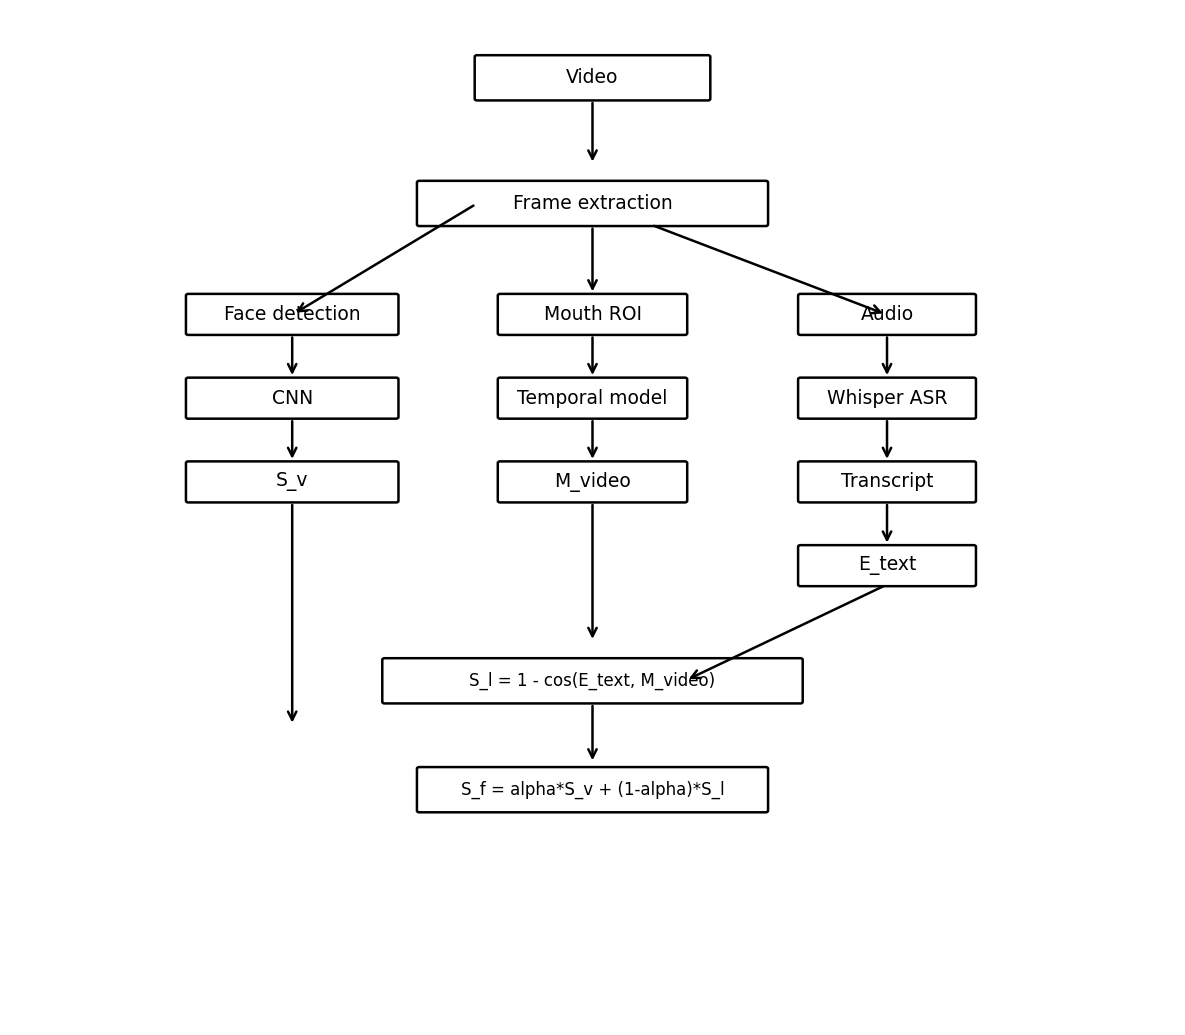
\includegraphics[width=0.75\linewidth]{figures/architecture.png}
  \caption{Proposed architecture: visual branch ($S_v$), sync branch ($S_l$ from $M_{\text{video}}$ and $E_{\text{text}}$), and fusion $S_f$.}
  \label{fig:arch}
\end{figure}

\section{Dataset and Protocol}
\textbf{Manipulation types.} We use: \emph{real\_sync} (authentic); \emph{fake\_sync\_shift} (audio shifted in time); \emph{fake\_content\_mismatch} (lip motion vs transcript mismatch); \emph{fake\_audio\_synthetic} (synthetic voice). This allows controlled study of which modality is violated.

\textbf{Splits.} Train/validation/test splits are \emph{speaker-disjoint}: each speaker appears in only one split, avoiding speaker-specific memorisation and giving a realistic measure of generalisation.

\textbf{Statistics.} Our dataset has 818 samples in total (20 speakers, speaker-disjoint splits): 578 train, 120 validation, 120 test. Manipulation types include real (authentic), sync\_shift (temporal offset), content\_mismatch, and synthetic\_audio. Experiments in this paper use synthetic/demo data generated with this protocol; validation on larger real Turkish or external data (e.g.\ AVLips) is left for future work.

\section{Experiments}
\textbf{Setup.} Visual branch: ResNet-18 backbone, binary consistency head. Sync branch: temporal mouth encoder and text encoder; $S_l = 1 - \cos(E_{\text{text}}, M_{\text{video}})$. Fusion: $S_f = 0.5\, S_v + 0.5\, S_l$. Training: 578 train, 120 val; we report on the 120 test samples (3 held-out speakers).

\textbf{Main results.} Table~\ref{tab:main} reports accuracy, precision, recall, F1, AUC, and EER on the test set. The decision threshold is set by ROC Youden index (maximising $TPR - FPR$) rather than a fixed 0.5, since score distributions often do not centre at 0.5. To refresh: \texttt{python run\_pipeline.py experiments} then \texttt{export\_results\_latex.py --split test}.

% Auto-generated. Run: python scripts/export_results_latex.py --split test
\begin{table}[htbp]
  \centering
  \caption{Test set results ($n=1649$).}
  \label{tab:main}
  \begin{tabular}{lcccccc}
    \toprule
    Model & Acc. & Prec. & Rec. & F1 & AUC & EER \\
    \midrule
    Visual only ($S_v$) & 0.315 & 0.000 & 0.000 & 0.000 & 0.499 & 1.000 \\
    Sync only ($S_l$) & 0.685 & 0.000 & 0.000 & 0.000 & 0.500 & 1.000 \\
    Fusion ($S_f$) & 0.315 & 0.000 & 0.000 & 0.000 & 0.499 & 1.000 \\
    \bottomrule
  \end{tabular}
\end{table}

\textbf{Ablation (optional).} Vary $\alpha \in \{0.25, 0.5, 0.75\}$ and report Fusion accuracy, AUC, and EER. Table values are generated by the project (\texttt{run\_ablation\_alpha.py}).
% Fusion alpha ablation. Run: python scripts/run_ablation_alpha.py --out paper/ablation_alpha.tex
\begin{table}[htbp]
  \centering
  \caption{Fusion ablation: effect of $\alpha$ in $S_f = \alpha S_v + (1-\alpha) S_l$.}
  \label{tab:ablation_alpha}
  \begin{tabular}{lccc}
    \toprule
    $\alpha$ & Acc. & AUC & EER \\
    \midrule
    0.25 & 0.315 & 0.499 & 1.000 \\
    0.5 & 0.315 & 0.499 & 1.000 \\
    0.75 & 0.315 & 0.499 & 1.000 \\
    \bottomrule
  \end{tabular}
\end{table}

\textbf{Limitations.} Small dataset size, single run (no variance), and/or synthetic-only data should be stated; future work: multiple seeds, real Turkish data, larger benchmarks.

\section{Conclusion}
We presented a multimodal pipeline for speech--visual consistency with a visual branch ($S_v$), a sync branch ($S_l$), and fusion ($S_f$). Controlled manipulation types and speaker-disjoint evaluation allow interpretable comparison of visual-only, sync-only, and fused models. Current results are on synthetic/demo data (818 samples, 20 speakers); extending to larger real Turkish or AVLips data and reporting variance over runs would strengthen the contribution.

\bibliographystyle{plain}
\bibliography{refs}
\end{document}
